\section{Chapter 5 - Formulation of NLPs}
\subsection{Thursday 02/20/2025}
\subsubsection{Chapter Introduction}
Generally, there are two types of nonlinear problems in relation to their constraints:
\begin{itemize}
    \item Unconstrained
    \item Constrained
\end{itemize}
This will introduce the chapter and the general material discussed. 
For NLPs, there are also convex and non-convex problems.
Convex problems are generally much easier to solve than non-convex problems.
There are tricks that can be employed to help solve and reduce the complexity of the algorithms.
A final portion of this chapter will go into specific NLPs in chemical engineering applications.

\subsubsection{NLPs}
The general form of an NLP is 
\begin{align}
  \text{minimize} & \quad f(x) \\
  \text{subject to} & \quad g(x) \leq 0 \\
  & \quad h(x) = 0
\end{align}
where any of the functions $f, g, h$ are non-linear and $\textbf{x} \in \mathbb{R}^n$.
The problem above is convex if both $f, g$ are convex and $h$ is an affine function that can be represented as $h(x)=Ax-b$.

In chemical engineering, there are a few sources of non-linearity:
\begin{itemize}
    \item $c = \alpha (size)^\beta $: Formula for cost of capital. This is a long term cost and generally marginally decreases with size, therefore $0 \leq \beta \leq 1$.
    \item $xy$: Splitter, which is a bilinear and non-convex term that takes an input and outputs the same amount by an amount of paths.
    \item $everything$: Thermodynamics, kinetics, transport, and other many chemical relations are not linear.
\end{itemize}

\subsubsection{Tricks}
Some tricks can be employed that alleviate constraints of chemistry or physics and give generally accurate convex approximations.
\begin{itemize}
    \item Bounds: $l \leq x \leq u$. These constrain the design variables to be in a well constrained area. A smaller design space is easier to explore.
    \item Linear: Try to approximate or represent things as linearly whenever possible. For example, a ratio constraint $\frac{x_i}{x_T} \leq \alpha \rightarrow x_i \leq \alpha x_T$.
    \item Elimination: Eliminating variables where possible. For example, a constraint $y = x_1 + x_2$ with those three variables can have the rest of the problem's $y$ replaced with $x_1 + x_2$.
\end{itemize}
The complexity of chemical engineering problems and formulating them as LPs can be seen in multiple paradigms.
\begin{itemize}
    \item Level of aggregation: Chemical engineering problems have many different unit operations that will compress, react, separate, etc different chemicals. These unit operations can be aggregated into different "zones"to assist with having linear constraints in between these zones. Effectively, simplifying the unit operations to reduce the amount of design variables.
\end{itemize}

\subsection{Tuesday 02/25/2025}
For a mixer, the only balance equations necessary are the input must equal the output.
\begin{center}
\begin{tikzpicture}
    \node[circle, draw, minimum size=1cm] (mixer) at (0,0) {Mixer};
    \draw[->] (-2,0) -- (mixer.west);
    \draw[->] (0,-2) -- (mixer.south);
    \draw[->] (mixer.east) -- (2,0);
\end{tikzpicture}
\end{center}
The chemical components that enter must equal the chemical components that exit this mixer.

\subsection{Thursday 02/27/2025}
Below is an example of a chemical layout with certain unit operations that perform operations on their inputs.
\begin{center}
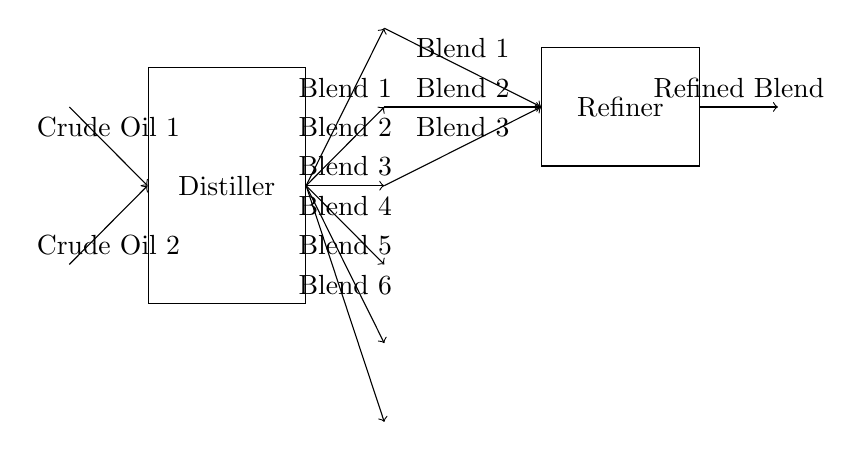
\begin{tikzpicture}
    \node[rectangle, draw, minimum width=2cm, minimum height=3cm] (distiller) at (0,0) {Distiller};
    \draw[->] (-2,1) -- (distiller.west) node[midway, above] {Crude Oil 1};
    \draw[->] (-2,-1) -- (distiller.west) node[midway, below] {Crude Oil 2};
    \draw[->] (distiller.east) -- (2,2) node[midway, above] {Blend 1};
    \draw[->] (distiller.east) -- (2,1) node[midway, above] {Blend 2};
    \draw[->] (distiller.east) -- (2,0) node[midway, above] {Blend 3};
    \draw[->] (distiller.east) -- (2,-1) node[midway, above] {Blend 4};
    \draw[->] (distiller.east) -- (2,-2) node[midway, above] {Blend 5};
    \draw[->] (distiller.east) -- (2,-3) node[midway, above] {Blend 6};
    
    \node[rectangle, draw, minimum width=2cm, minimum height=1.5cm] (refiner) at (5,1) {Refiner};
    \draw[->] (2,2) -- (refiner.west) node[midway, above] {Blend 1};
    \draw[->] (2,1) -- (refiner.west) node[midway, above] {Blend 2};
    \draw[->] (2,0) -- (refiner.west) node[midway, above] {Blend 3};
    \draw[->] (refiner.east) -- (7,1) node[midway, above] {Refined Blend};
\end{tikzpicture}
\end{center}
The outputs of this system are petrol 1, petrol 2, jet fuel, fuel oil, and lube.